%%%%%%%%%%%%%%%%%%%%%%%%%%%%%%%%%%%%%%%%%%%%%%%%%%%%%%%%%%%%%%%%%%%%%%%%%%%%%%%%%%%%
% Document data
%%%%%%%%%%%%%%%%%%%%%%%%%%%%%%%%%%%%%%%%%%%%%%%%%%%%%%%%%%%%%%%%%%%%%%%%%%%%%%%%%%%%
\documentclass[12pt]{article} %report allows for chapters
%%%%%%%%%%%%%%%%%%%%%%%%%%%%%%%%%%%%%%%%%%%%%%%%%%%%%%%%%%%%%%%%%%%%%%%%%%%%%%%%%%%%
\usepackage{preamble}

\begin{document}

\begin{center}
   \textsc{\large MATH 271, Homework 2, \emph{Solutions}}\\
   \textsc{Due September 13$^\textrm{th}$}
\end{center}
\vspace{.5cm}

\begin{problem}
    Solve the following autonomous equation.
    \[
    x'=-x^2.
    \]
    Can $x(0)=0$ be an initial condition?
\end{problem}
\begin{solution}
We have seen this equation arise from studying chemical reactions.  Specifically, this equation could model
\[
2x \xrightarrow{k=1} \to \textrm{Products}.
\]
This equation is also separable.  Which means we can solve by
\begin{align*}
    x'=\frac{dx}{dt}&=-x^2\\
    \iff -\frac{dx}{x^2}&=dt.
\end{align*}
We can then integrate both sides to find
\[
\frac{1}{x}=t+C.
\]
Then we solve for $x$ to find our general solution
\[
\boxed{x=\frac{1}{t+c}.}
\]
Since this equation could model the above reaction, we should expect that the initial condition of $x(0)=0$ works. Why is that? If we start with no reactants (i.e., this initial condition), then no reaction should occur!  We can see that by noting
\[
x'(0)=-x(0)^2=0
\]
which shows that $x'(0)=0$ given this initial condition.  In that case the solution is trivial and no dynamics occur.

However, just by looking at solving the equation we have from our general solution
\[
x(0)=\frac{1}{0+c}=\frac{1}{c}
\]
it is not really possible to solve this equation. However, if we consider something like the $\lim_{c\to \infty} \frac{1}{t+c}=0$ then this may make some sense.  Below is a graph of many different values of $c$. Notice that they approach the case $x(t)=0$ as a solution as $t\to \infty$. So in the case that $x(0)=0$ the particular solution would be
\[
\boxed{x(t)=0.}
\]
\begin{figure}[H]
    \centering
    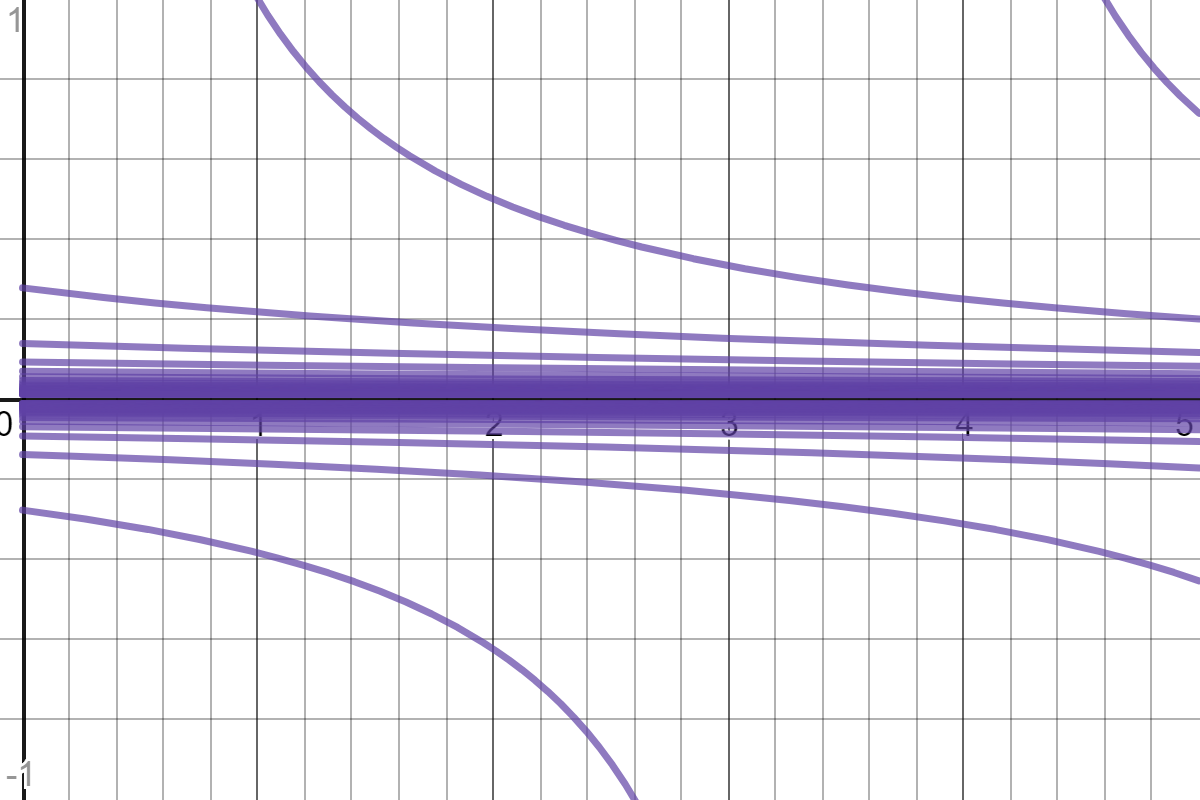
\includegraphics[width=\textwidth]{2nd_order_chem.png}
\end{figure}
\end{solution}

\newpage
\begin{problem}
Objects near Earth fall due to gravity.  The acceleration of an object due to gravity is then
\[
x''=g,
\]
where $x$ represents the distance above the ground and $g\approx -9.8\frac{m}{s^2}$.  
\begin{enumerate}[(a)]
    \item Find the general solution to the equation.
    \item Given the initial data $x(0)=0$ and $x'(0)=1$, find the particular solution.
    \item Plot your solution over a meaningful range of time.
    \item When is the object touching the ground?
\end{enumerate}

\end{problem}
\begin{solution}~
\begin{enumerate}[(a)]
    \item This equation can be solved by integrating twice.  However, I like to make a substitution of $y=x'$ so that we can write
    \[
    y'=g.
    \]
    Now, this is a first order separable equation which we can solve by
    \begin{align*}
        \frac{dy}{dt}&=g\\
        \int dy&= \int gdt\\
        y&= gt+C_1.
    \end{align*}
    Now, since $y=x'$ we can look at
    \[
    x'=gt+C_1
    \]
    which is also separable.  We integrate and find
    \begin{align*}
        \frac{dx}{dt}&=gt+C_1\\
        \int dx &= \int gt+C_1 dt\\
        x(t)&= \frac{1}{2}gt^2+C_1t+C_2
    \end{align*}
    is our general solution.
    \item Now, we use our initial data along with our general solution
    \begin{align*}
        0=x(0)&=\frac{1}{2}g(0)^2+C_1(0)+C_2\\
        &=C_2.
    \end{align*}
    So $C_2=0$. Next, use the information about the first derivative $x'(0)=1$ and we have
    \begin{align*}
        1=x'(0)&=g(0)+C_1\\
        =C_1.
    \end{align*}
    Thus $C_1=1$. Now, our particular solution is
    \[
    \boxed{x(t)=\frac{1}{2}gt^2+t.}
    \]
    \item Here's a plot of the solution from time $t=0$ until it hits the ground (see (d)).
    \begin{figure}[H]
        \centering
        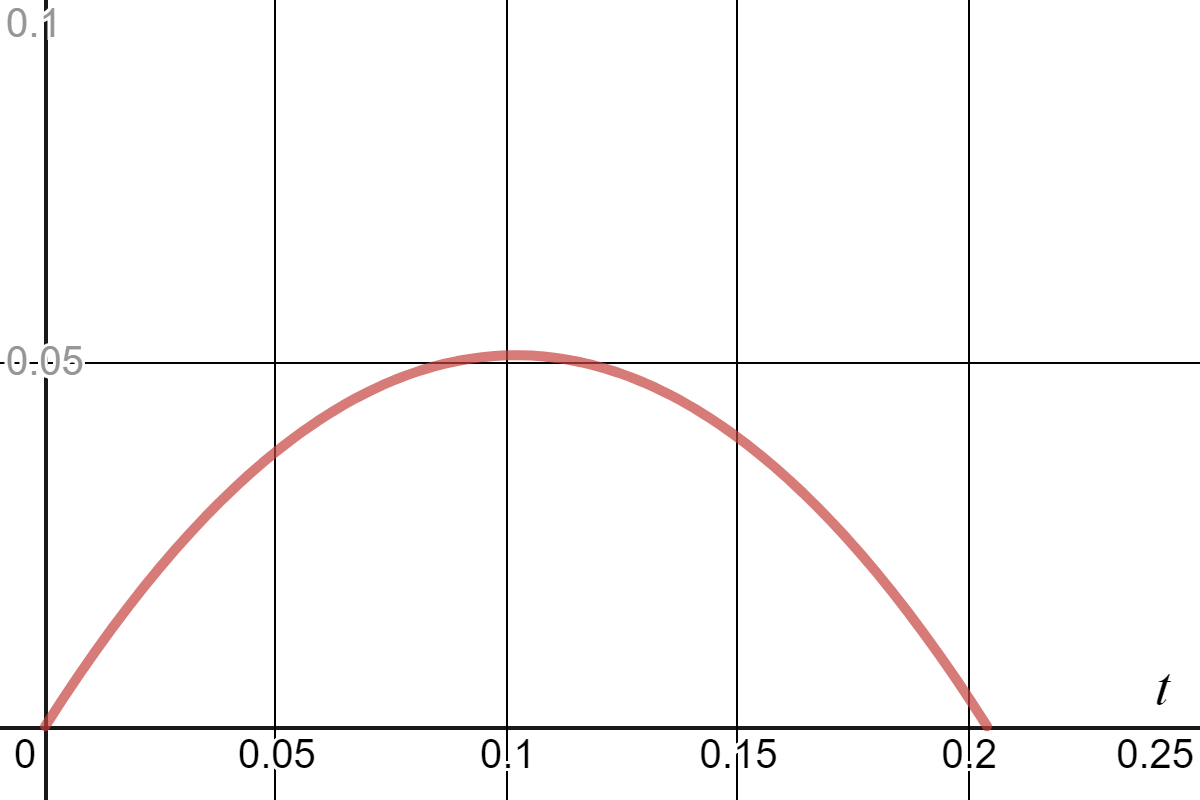
\includegraphics[width=\textwidth]{projectile.png}
    \end{figure}
    \item This was maybe better to think about before plotting in (c)! Now, the points at which the object is on the ground are the values of $t$ where $x(t)=0$ since $x$ represents the height above the ground.  So we have to solve
    \[
    0=x(t)=\frac{1}{2}gt^2+t=t\left(\frac{1}{2}gt+1\right).
    \]
    This has roots $t=0$ and $t=-\frac{2}{g}$
\end{enumerate}
\end{solution}


\newpage
\begin{problem}
Consider the following differential equation.
\[
x' = x\cos(t).
\]
\begin{enumerate}[(a)]
    \item What is the order of this equation?
    \item Find the general solution to this equation.
    \item Given the initial data $x(0)=1$, find the particular solution.
    \item Plot this function and explain in words what the solution represents if $x(t)$ is position.
\end{enumerate}
\end{problem}
\begin{solution}~
\begin{enumerate}[(a)]
    \item This is a first order equation that is also separable.
    \item We can find the general solution by 
    \begin{align*}
        \frac{dx}{dt}&= x\cos(t)\\
        \int \frac{1}{x}dx &= \int \cos(t)dt\\
        \ln(x)&=\sin(t)+C.
    \end{align*}
    Then we solve for $x$ to find
    \begin{align*}
        x&=e^{\sin(t)+C}=e^C \cdot e^{\sin(t)}\\
        &= Ae^{\sin(t)},
    \end{align*}
    which is our general solution.
    \item If we have $x(0)=1$ then we plug this into our general solution
    \[
    1=x(0)=Ae^{\sin(0)}=A
    \]
    so that $A=1$. Thus the particular solution is
    \[
    \boxed{x(t)=Ae^{\sin(t)}.}
    \]
    \item The solution represents a system that oscillates back and forth. However, it is not oscillion as we see with a Hookean spring and a mass system.  In this case, this would a oscillation due to something else entirely. Here is a plot of the solution.
    \begin{figure}[H]
        \centering
        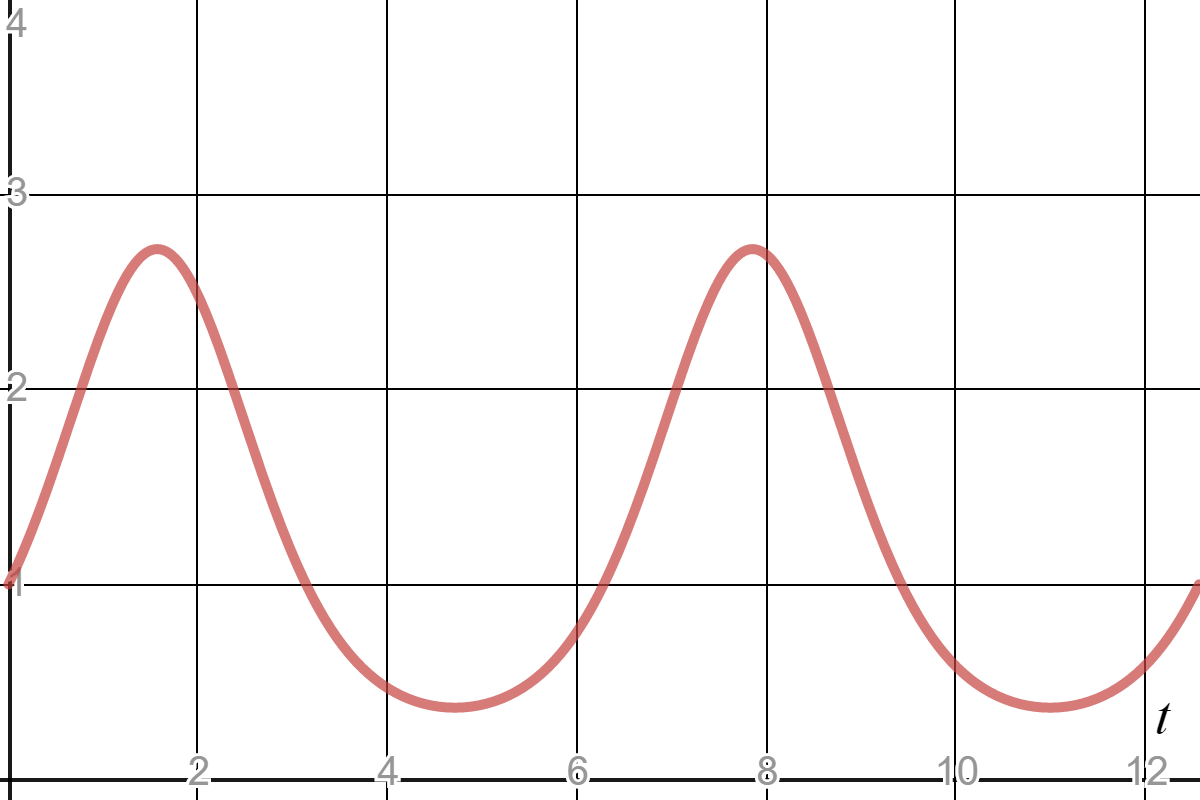
\includegraphics[width=\textwidth]{esint.png}
    \end{figure}
\end{enumerate}
\end{solution}

\newpage
\begin{problem}
Consider the differential equation
\[
x'=\frac{x+t}{t}.
\]
\begin{enumerate}[(a)]
    \item Let $f(x,t)=\frac{x+t}{t}$. Show that $f(x,t)=f(\lambda x, \lambda t)$.
    \item Given (a) holds, use the change of variables $u=\frac{x}{t}$ to rewrite the differential equation as a separable equation in terms of $u$.
    \item Find the general solution to the equation and write your solution in terms of the original variables $t$ and $x$.
\end{enumerate}
\end{problem}
\begin{solution}~
\begin{enumerate}[(a)]
    \item To show this, we check to see if the equality is true by 
    \begin{align*}
        f(\lambda x, \lambda t) &= \frac{\lambda x + \lambda t}{\lambda t}\\
        &= \frac{\lambda(x+t)}{\lambda t}\\
        &= \frac{x+t}{t}\\
        &= f(t).
    \end{align*}
    So the property holds, which leads us to (b).
    \item Now, we let $u=\frac{x}{t}$ which allows us to say $x=tu$.  We can then take
    \[
    x' = f(x,t) = f(tu,t)=\frac{tu+t}{t}=\frac{t(u+1)}{t}=u+1.
    \]
    Given our substitution, we can also take
    \[
    x'=(tu)'=u+tu'
    \]
    and substitute this back in our other expression to get
    \[
    u+tu'=u+1.
    \]
    We can simplify this a bit
    \begin{align*}
        u+tu'&=u+1\\
        tu'&= 1\\
        u'&=\frac{1}{t}.
    \end{align*}
    This is a separable equation.
    \item Now we can solve the previous equation using separation. So we have
    \begin{align*}
        \frac{du}{dt}&= \frac{1}{t}\\
        \int du &= \int \frac{dt}{t}\\
        u&= \ln(t)+C.
    \end{align*}
    Recall that we let $u=\frac{x}{t}$ and to get back to the original variable we need to solve for $x$. So we take
    \begin{align*}
        u=\frac{x}{t}&=\ln(t)+C\\
        x&=t\ln(t)+Ct.
    \end{align*}
    So the general solution to our original equation is
    \[
    \boxed{x(t)=t\ln(t)+Ct.}
    \]
\end{enumerate}
\end{solution}

\newpage
\begin{problem}
Find the general solution to the following equation.
\[
tx'+2x=\frac{\sin(t)}{t}.
\]
Show that your solution is correct. (\emph{Hint: can you use an integrating factor?})
\end{problem}
\begin{solution}
Note that this is a first order linear equation if we divide the whole expression by $t$. We can see this by,
\begin{align*}
    tx'+2x&=\frac{\sin(t)}{t}\\
    x'+\frac{2}{t}x&=\frac{\sin(t)}{t^2}.
\end{align*}
This matches the form of a first order linear equation which is typically written as
\[
x'+f(t)x=g(t).
\]
So note that in our case, $f(t)=\frac{2}{t}$ and $g(t)=\frac{\sin(t)}{t^2}$. Given that, we can solve this equation using the integrating factor technique.  For that, we have the integrating factor
\begin{align*}
\mu &= e^{\int f(t)dt}\\
&=e^{\int \frac{2}{t}dt}\\
&= e^{2\ln(t)}\\
&=e^{\ln\left(t^2\right)}\\
&=t^2.
\end{align*}
Now, we have $\mu$ and we can find $x(t)$ by
\begin{align*}
    x&= \frac{1}{\mu(t)}\int \mu(t)g(t)dt\\
    &= \frac{1}{t^2} \int t^2 \frac{\sin(t)}{t^2}dt\\
    &= \frac{1}{t^2}\int \sin(t)dt\\
    &= -\frac{1}{t^2} \cos(t)+\frac{C}{t^2}.
\end{align*}
So our general solution is
\[
\boxed{x(t)=-\frac{1}{t^2}\cos(t)+\frac{C}{t^2}.}
\]
\end{solution}

\end{document}